\section{Results and discussion: The axial mass effect}
Figure~\ref{CountRate} demonstrates the result of our calculation: the relative contributions to the electron-like and muon-like event rates caused by the QES interactions with hydrogen and oxygen nuclei in the Super-Kamiokande detector. Evaluations were done with several values of nucleon axial mass and normalized to one of them. As you can see, the adequate choice of the axial mass value is very important to the neutrino event rate calculations.

\begin{figure}[h!]
\begin{center}
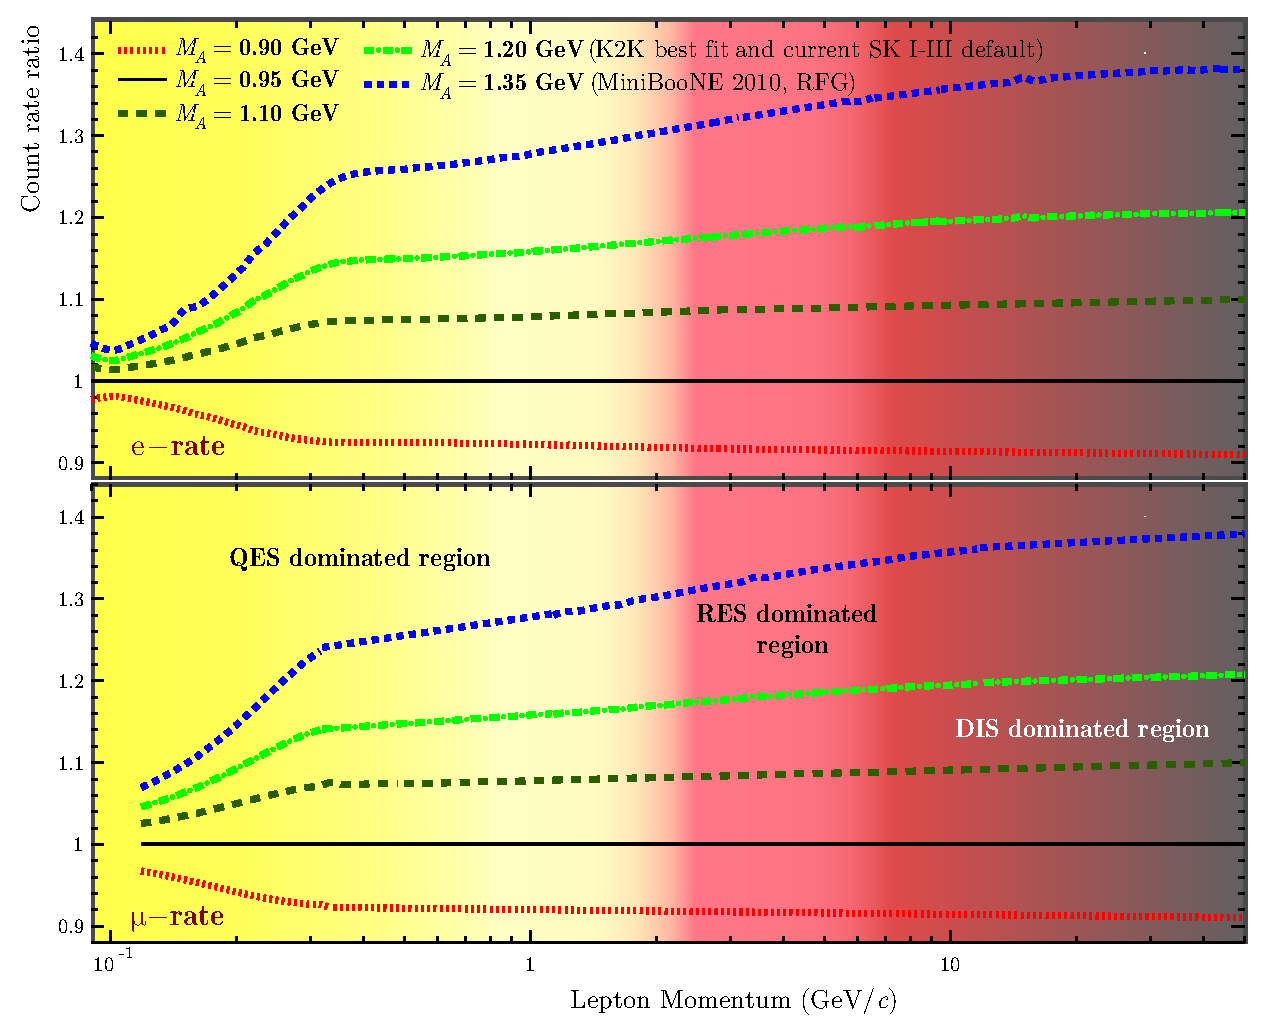
\includegraphics[width=0.45\textwidth]{./SK/Count_rate_ratio.eps}
\caption{\label{CountRate}Electron and muon count rates in the Super-Kamiokande detector due to QES interactions evaluated with different values of $M_A$ and normalized to one of them. The calculations are done for the normal neutrino mass hierarchy. Energy regions, where quasielastic, resonant or deep inelastic scattering are dominant, are shown approximate}
\end{center}
\end{figure}

A nuclear model commonly used in experiments for data processing is the Relativistic Fermi Gas model. All of experimantal data mentioned in Introduction were obtained by using this model. Applying another model could essentially modify extracted values. Figure~\ref{MiniBooNE} shows calculation exploiting the nuclear model of Martini \textit{et al.}~\cite{Martini:2011wp}, which yields $M_A$ compatible with our best-fit value. The natural conclusion is that the Relativistic Fermi Gas model does not work in the low-energy region. The problem is that we don't have nuclear model, which works properly for all energies. Therefore, even in case we knew the correct value of the axial mass, we could not use it.

But finally, we have an idea of how to avoid this difficulty. As we know, using the RFG model with different values of $M_A$ can give a good description of experimental data obtained in different energy ranges. Thus, we propose to continue using the Relativistic Fermi Gas model but modify the axial form factor to compensate nuclear effects in the low-energy region. For this parametrization we need to introduce variable effective axial mass:
\begin{equation}
F_{A}^{\mathrm{eff}}(Q^{2},E_{\nu})=g_{A}\left(1+\frac{Q^{2}}{(M_{A}^{\mathrm{eff}}(E_{\nu}))^{2}}\right)^{-2}.
\end{equation}
Figure~\ref{MA_QES_Effective} demonstrates very schematically how we can fit experimental data to get $M_{A}^{\mathrm{eff}}$. In the near future we plan to perform a global statistical analisys to adjust $M_{A}^{\mathrm{eff}}$.

\begin{figure}[h!]
\begin{center}
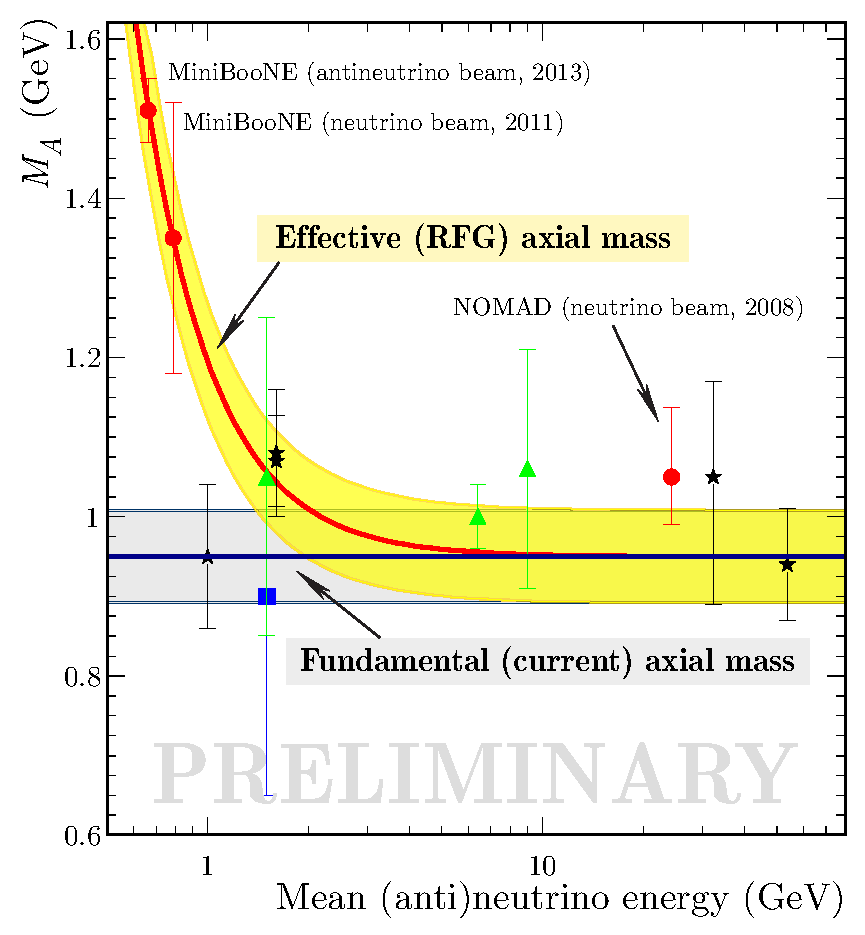
\includegraphics[width=0.45\textwidth]{./QES/MA_QES_Effective-2.eps}
\caption{\label{MA_QES_Effective}The concept of how we can fit experimental data to get $M_{A}^{\mathrm{eff}}$. Only selected experimental points are shown. Only MininBooNE data are used to fit the $M_{A}^{\mathrm{eff}}$ curve}
\end{center}
\end{figure}

In contrast, we propose to call constant $M_A$ used in real form-factor $F_A$ ``current''. Figure~\ref{EventRates} displays ratios of the neutrino event rates evaluated with several values of current $M_A$ to ones computed with preliminary offered $M_{A}^{\mathrm{eff}}$.

\begin{figure}[h!]
\begin{center}
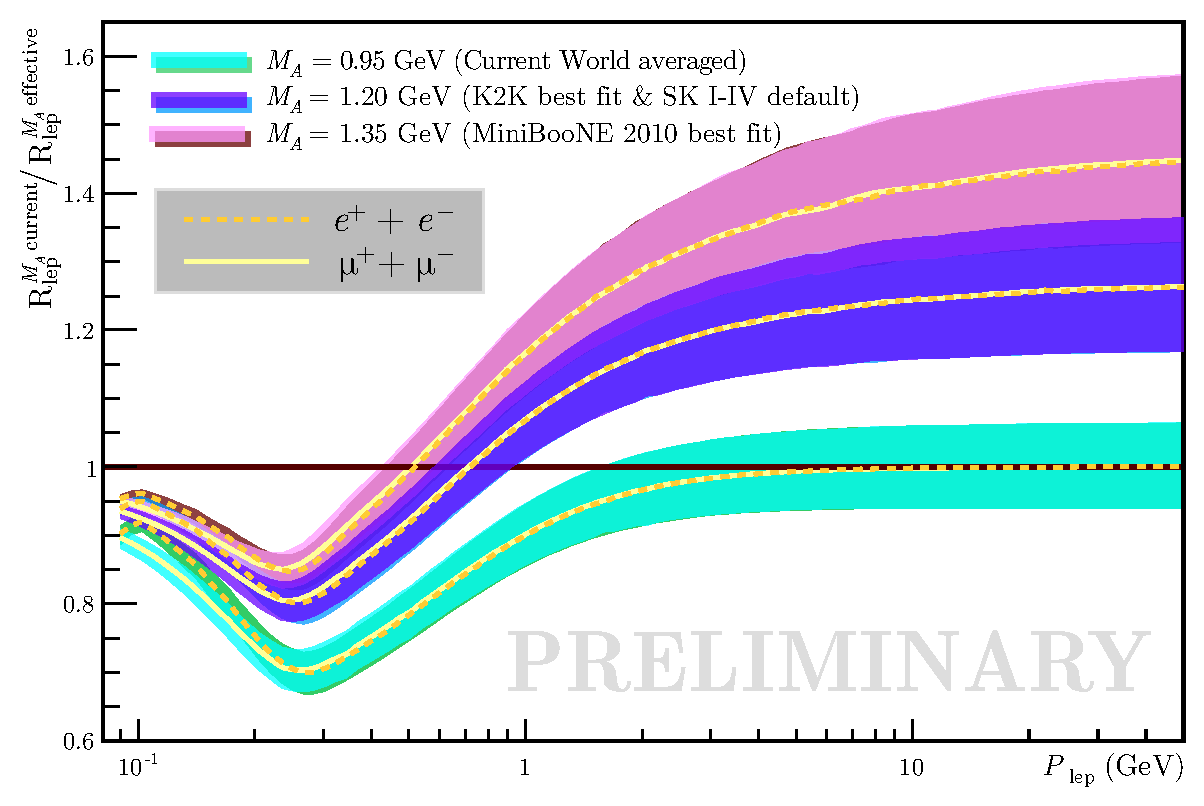
\includegraphics[width=0.45\textwidth]{./SK/cvsv2lmn_all2.eps}
\caption{\label{EventRates}Electron-like and muon-like event rates caused by the QES interactions in the SK detector. The rates are evaluated with several values of current $M_A$ and normalized to the rates calculated with the effective $M_A$. The calculations are done for the normal neutrino mass hierarchy}
\end{center}
\end{figure}
